
\section{Evaluation}
\label{sec:eval}

We further compare the performance of \sys against the original \libfuzzer and the popular grey-box fuzzer AFL~\cite{AFL}.
We select test cases from fuzzer-test-suite~\cite{fuzzer-test-suite} as the test cases, which a set of test cases for fuzzing engines provided by Google.
The selected test cases are \ttstyle{CVE-2016-5180}, \ttstyle{CVE-2015-8317} and \ttstyle{HeartBleed (CVE-2014-0160)}.
To work the \sys, we slightly modify the test cases if they do not implement a \ttstyle{main} function but only implement the \ttstyle{LLVMFuzzerTestOneInput} function.
An additional \ttstyle{main} function is added to the test case to read test inputs from standard input and pass read inputs via the \ttstyle{LLVMFuzzerTestOneInput} function.
%
We perform the evaluations on a virtual server hosted on Google cloud platform. The virtual server use the \ttstyle{n1-standard-1} configuration (single vCPU, 3.75GB RAM).

%In order to work with \sys, we modify the \texttt{target.cc} in some test cases. Take \texttt{c-ares-CVE-2016-5180} for example, we modified the \texttt{extern "C" int LLVMFuzzerTestOneInput(const uint8\_t *Data, size\_t Size)} function declaration to \texttt{int main()}. And use \texttt{read} function to read input data, the size is the length of input data. Check out more detail of patching fuzzer-test-suite in wiki page of our repository. The following specification is our machine information and all experiments were performed on it.
%
%\begin{lstlisting}
%virtual private server on Google Cloud Platform
%n1-standard-1 (one vCPU, 3.75 GB RAM)
%\end{lstlisting}

\subsection{Correctness}

We evaluate the correctness of \sys by comparing the results with those from the original \libfuzzer.
Compared to the original \libfuzzer, we can successfully find the vulnerabilities from the first two test cases.
Although \sys is able to generate inputs that crash the test case, it fails to find the vulnerability because of the lack of address sanitizer hooks.
%
Figure~\ref{fig:libfuzz} shows the performance numbers for the three test cases. It shows that the dynamical instrumentations performed by \sys is about 3x to 6x slower than static instrumentation in native programs.

\begin{figure}
\centering
%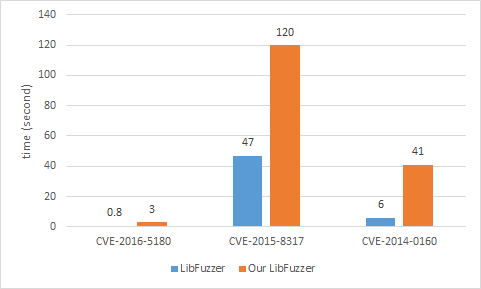
\includegraphics[width=\linewidth]{eval1.png}
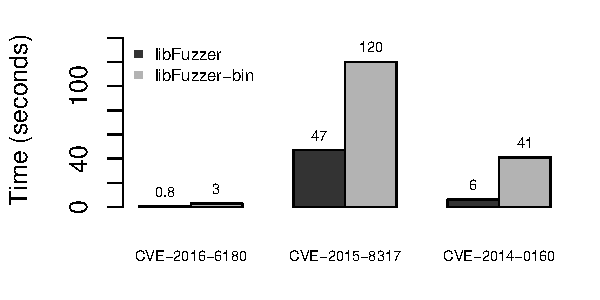
\includegraphics[width=.90\columnwidth]{eval_libfuzz.pdf}
\caption{Performance Comparison for native \libfuzzer and \sys.}
\label{fig:libfuzz}
\end{figure}

%We choose some CVE test cases in fuzzer-test-suite, including \texttt{CVE-2016-5180}, \texttt{CVE-2015-8317} and \texttt{HeartBleed (CVE-2014-0160)}, to evaluate the performance of our LibFuzzer. These are the output of running test cases by our LibFuzzer and do it 10 times to calculate the average time.
%
%\begin{enumerate}
%    \item [1.] \texttt{CVE-2016-5180}
%\end{enumerate}
%
%This is a 1-byte-write-heap-buffer-overflow in c-ares. This bug was one of out a chain of two bugs that made a ChromeOS exploit possible: code execution in guest mode across reboots.
%
%\begin{lstlisting}
%#0      READ units: 1
%#2      INITED cov: 4 ft: 20 corp: 1/1b exec/s: 2 rss: 25Mb
%#3      NEW    cov: 4 ft: 39 corp: 2/3b exec/s: 3 rss: 25Mb L: 2/2 MS: 1 CopyPart-
%#4      pulse  cov: 4 ft: 59 corp: 2/3b exec/s: 2 rss: 25Mb
%#4      NEW    cov: 4 ft: 59 corp: 3/5b exec/s: 2 rss: 25Mb L: 2/2 MS: 2 CopyPart-ShuffleBytes-
%Error status : 139
%Signal : Segmentation fault
%\end{lstlisting}
%
%And we can find the 1-byte-write-heap-buffer-overflow by our LibFuzzer within 3 seconds.
%
%\begin{enumerate}
%    \item [2.] \texttt{CVE-2015-8317}
%\end{enumerate}
%
%This is a 1-byte-read-heap-buffer-overflow and a memory leak in libxml2.
%
%\begin{lstlisting}
%#0      READ units: 1
%Error status : 139
%Signal : Segmentation fault
%\end{lstlisting}
%
%Using our LibFuzzer can find the 1-byte-read-heap-buffer-overflow and a memory leak within 120 seconds.
%
%\begin{enumerate}
%    \item [3.] \texttt{HeartBleed (CVE-2014-0160)}
%\end{enumerate}
%
%This is a multi-byte-read-heap-buffer-overflow in openssl.
%
%\begin{lstlisting}
%#0      READ units: 1
%...
%Error status : 134
%Signal : Aborted
%\end{lstlisting}
%
%In this test case, we cannot find the multi-byte-read-heap-buffer-overflow because this is a network service and there are a few asserts cannot pass by running program in local. As a result, we only got an aborted signal, not segmentation fault.
%
%Compared with original LibFuzzer and plot the chart.
%
%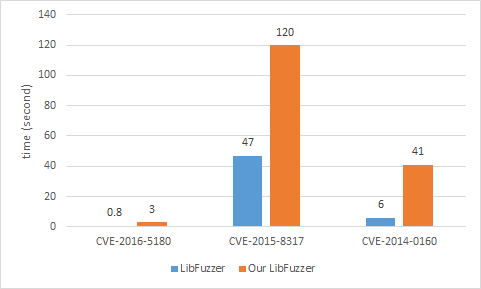
\includegraphics[width=\linewidth]{eval1.png}
%
%As we can see, because of the implementation of our LibFuzzer, the IO speed and analysis take a lot of time. And the performance is slower than original LibFuzzer. But compared the time of original LibFuzzer and our LibFuzzer took, we still can find the bugs efficiently in these test cases.

\subsection{Performance}

We also compare the performance of \sys against that of AFL QEMU mode, which also works for fuzzing binaries.
According to the statements from AFL document, running AFL in QEMU mode incurs roughly 2x to 5x overheads compared to that without instrumentation.
We measure the performance overhead by comparing the running time of a program with and without instrumentation.
Figure~\ref{fig:afl} shows the overheads measured from \sys. It shows that our design and implementation is efficient and competitive to that of AFL.
Note that AFL fails on running the test cases for CVE-2014-0160, so an ``N/A" is marked on that bar.

\begin{figure}
\centering
%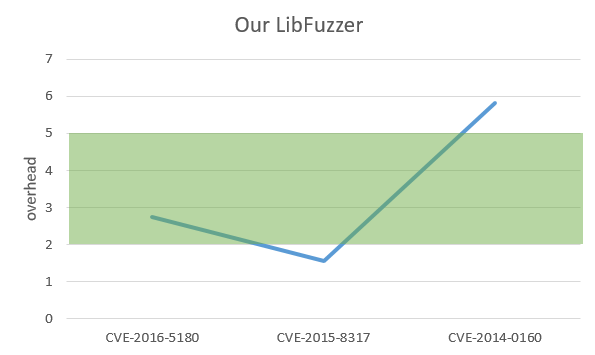
\includegraphics[width=\linewidth]{eval2.png}
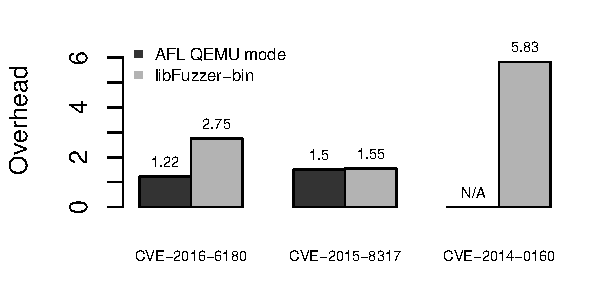
\includegraphics[width=.90\columnwidth]{eval_afl.pdf}
\caption{Performance comparison against AFL.}
\label{fig:afl}
\end{figure}

